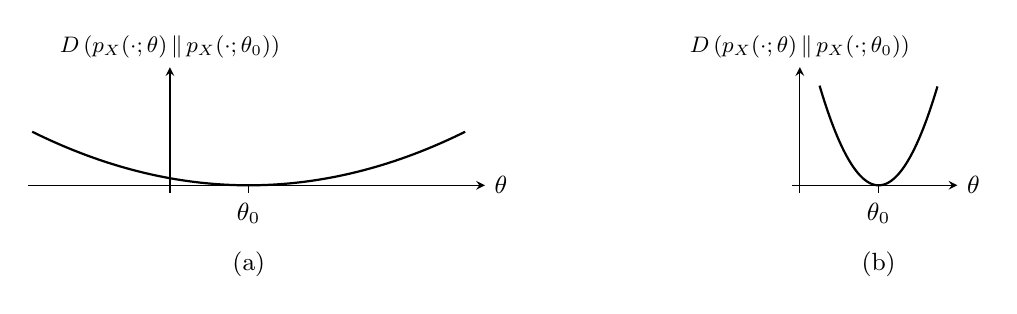
\begin{tikzpicture}
\shorthandoff{>}
%
\pgfmathsetmacro{\t}{1}
\pgfmathsetmacro{\dx}{8}
%
% peque�a curvatura
\draw[>=stealth,->] (-1.8,0)--(4,0) node[right]{\small $\theta$};
\draw[>=stealth,->] (0,-.1)--(0,1.5) node[above,scale=.9]{\small $D\left( p_X(\cdot;\theta) \, \| \, p_X(\cdot;\theta_0) \right)$};
\draw[thick,domain=-1.75:3.75,samples=200] plot (\x,{.09*abs(\x-\t)^2});
\draw (\t,0)--(\t,-.1) node[below]{\small $\theta_0$};
%
% granda curvatura
\draw[>=stealth,->] ({-.1+\dx},0)--({2+\dx},0) node[right]{\small $\theta$};
\draw[>=stealth,->] (\dx,-.1)--(\dx,1.5) node[above,scale=.9]{\small $D\left( p_X(\cdot;\theta) \, \| \, p_X(\cdot;\theta_0) \right)$};
\draw[thick,domain=.25:1.75,samples=200] plot ({\x+\dx},{2.25*abs(\x-\t)^2});
\draw ({\t+\dx},0)--({\t+\dx},-.1) node[below]{\small $\theta_0$};
%
\draw (\t,-1) node{\small (a)};
\draw ({\t+\dx},-1) node{\small (b)};
\end{tikzpicture}